%% ------------------------------------------------------- %%
%% Rodin
%% ------------------------------------------------------- %%
\section{Titre}
Presenter ici succinctement Event-B et la plate-forme Rodin.

Preciser que le code se trouve sous SourceForge et donner le chemin d'acces.

\subsection{Titre}
Contribution d'un plug-in SMT pour la plate-forme Rodin.

\begin{figure}
\centering
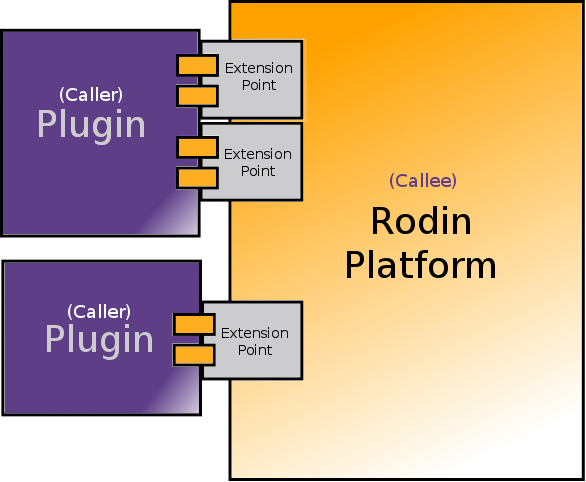
\includegraphics[scale=0.5]{Rodin.png}
\caption{Contributing to the Rodin platform} 
\label{Fig:Rodin Platform}
\end{figure}

La plate-forme Rodin est extensible.
\begin{itemize}
\item Plug-ins.
\item Points d'extensions.
\end{itemize}
Plus precis�ment, il est possible d'ajouter de nouveaux raisonneurs.
\begin{itemize}
\item En entree : un sequent Hypotheses |- But.
\item Branchement � un prouveur SMT.
\item En sortie : une r�gle de preuve.
\end{itemize}

\subsection{Titre}
Branchement a un Prouveur SMT.

\begin{figure}
\centering
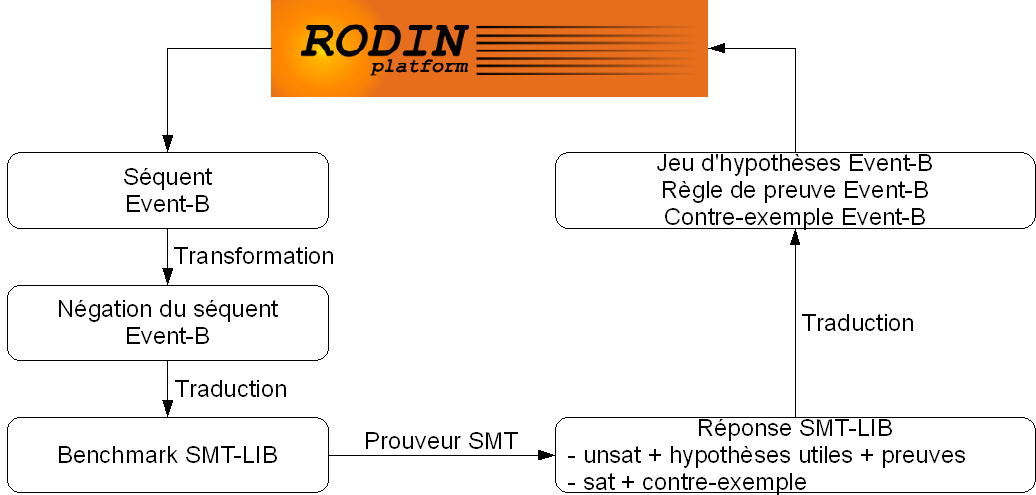
\includegraphics[scale=0.5]{Branchement_SMT.png}
\caption{Connecting an SMT solver} 
\label{Fig:SMT solver}
\end{figure}

Etant donne que l'on fait appel � un prouveur SMT, il est necessaire, afin de verifier la satisfaisabilite d'un lemme Event-B, de passer la negation de ce lemme au prouveur.
Si la negation du lemme n'est pas satisfaisable, le lemme original est valide.

Les etapes de traduction sont les etapes les plus delicates. Elles englobent plusieurs sous-taches qui vont permettre de selectionner les hypotheses, determiner quel format SMT-LIB generer (en fonction du prouveur appele, de la version SMT-LIB supportee, des theories supportees, etc), conserver un lien entre un jeu d'hypotheses au format Event-B et des hypotheses au format SMT-LIB.